% !TEX encoding = UTF-8
% 第五章（解读）：控制端——预测器不是执行器（C1/C2/C3）
% 对应论文 §5 开场、§5.1（C1/C2 范数帽）、§5.2（C3 秩-1 plant）与 Algorithm 1。
% §5.3 见解读第六章（ch06）；§5.4--§5.6 见解读第七章（ch07）；§5.7 见解读第八章。

\section{控制端：预测器不是执行器（C1/C2/C3）}
\label{sec:ch05}

\begin{keybox}{本章速览}
\begin{itemize}
  \item 论文 §5 按\textbf{失败模式}而非按方法组织控制实验：由 proxy 驱动的帽
        （C1/C2）动不了 $\lmax$；秩-1 plant（C3）两种体制都不下逃逸；
        只有 SAM 的全局动作把均衡点压下去。
  \item C1 权重范数帽（norm cap，把权重范数投影回预算球的干预；plain 网）：约 $750/3000$ 步触发，
        $\lmax^{\mathrm{final}}=40.26\pm0.43=2/\eta$，无逃逸。
  \item C2 $\gamma$-帽（BN 网）：$\lmax^{\mathrm{final}}=81.6\pm19.2$
        vs 基线 $73.0\pm12.9$，无逃逸，精度还略差（$0.754$ vs $0.768$）。
  \item C3 秩-1 阻尼：滞后 $\hat v$ 钉在 $2/\eta$（体制 (i)，
        $40.12\pm0.12$）；精确 $\hat v$ 上逃逸到 $261.8\pm5.4$
        （体制 (ii)）——两个结局都背向控制目标。
  \item 只有 SAM 全局扰动下行：$21.35\pm0.04<40$。
\end{itemize}
\end{keybox}

\paragraph{本章在论文中的位置。}
论文的核心论点``sharpness proxy 是预测器、不是执行器''，其前半（预测端）已在
论文第 2--4 节站稳了脚跟；从 §5 开始转向控制端，问的是反过来的
问题：能否用这些便宜的 proxy（或它们指向的曲率信息）\emph{驱动}训练离开 EoS
均衡点（``点''是行文习惯——均衡实指那条 $\lmax\approx2/\eta$ 的
周期-2 振荡轨道，见第九章）？本章覆盖论文 §5 的开场、§5.1（C1/C2 两个范数帽控制）与 §5.2（C3
秩-1 plant——论文自称``最干净的实验''），并转述 Algorithm 1 的逻辑。§5.3
（SAM 逃逸与 X-SAM 消融）在解读第 \ref{sec:ch06} 章；§5.4--§5.6 的三个压力
测试（谱迁移反驳、正交阻尼与传感滞后、clamp-free 桥）在第 \ref{sec:ch07}
章；第四个压力测试——ResNet-18/CIFAR-100 规模复现（§5.7）——留给解读第八章。

\subsection{组织逻辑：按失败模式排列的控制实验}
\label{sec:ch05-organization}

回忆引言里把``用 sharpness proxy 造优化器''拆成的两问：\textbf{预测/监控}
（proxy 是否跟踪 $\lmax$——是）与\textbf{控制/驱动}（proxy 能否把训练推离
$2/\eta$ 均衡——否）。§5 的实验排布不是按``试了哪些方法''罗列，而是按
\emph{失败模式}分成三类，每一类排除一种候选执行器：

\begin{enumerate}
  \item \textbf{由 proxy 驱动的帽（C1、C2，§5.1）}：把 proxy 本身（plain 网
        的权重范数、BN 网的 $\gamma$）投影住，看 $\lmax$ 是否跟着走。
        结果：不动。
  \item \textbf{秩-1 plant（C3，§5.2）}：不再约束 proxy，而是直接改写梯度
        ——与 SAM 同类的 plant 干预（直接改写梯度的执行器干预）。结局由
        特征向量估计 $\hat v$ 的精度决定，两种体制都不下逃逸：不完美阻尼
        留下自稳定帽（钉在 $2/\eta$，体制 (i)）；精确阻尼移除帽
        （上逃逸，体制 (ii)）。
  \item \textbf{全局动作（SAM，§5.3）}：唯一把均衡点压到阈值以下的。
\end{enumerate}

这个排序要成立，必须扛过四个压力测试，分别堵住四种替代解释：
``锐度其实搬到了未阻尼的方向''（谱迁移，§5.4$\to$\ref{sec:ch07}）；
``你阻尼错了方向/传感器太旧''（正交阻尼与滞后，§5.5$\to$\ref{sec:ch07}）；
``执行器根本没开火，是钳位休眠''（clamp-free 桥，§5.6$\to$\ref{sec:ch07}）；
``小 MLP 怪癖''（规模复现，§5.7$\to$解读第八章）。

术语提醒（与论文术语表一致）：\textbf{下逃逸}（flat-escape）$=$ 把 $\lmax$
严格压到阈值以下——声明的控制目标；\textbf{上逃逸}（sharp-escape）$=$ 帽被
移除后冲过阈值向上；\textbf{自稳定帽} $=$ $2/\eta$ 这个由周期-2 EoS 振荡
维持的自稳定上限；\textbf{有动作仍被钉住}（pinned despite action）$=$ 执行
器全力开火（实测、非休眠）而 $\lmax$ 仍留在跨种子噪声包络内——这是规模实验
（§5.7）的现象，第八章展开。

\subsection{C1/C2：帽住 proxy 本身，$\lmax$ 不跟}
\label{sec:ch05-normcaps}

设计动机直白：论文前半篇证明了这些零计算量的 proxy 在监控意义上可用
（plain 网 $\to\|\mathbf{W}\|$、BN 网 $\to\gamma$）。最自然的``控制化''就是
把 proxy 本身帽住——如果 proxy 与 $\lmax$ 的耦合是双向的，帽住 proxy 应该
连带把 $\lmax$ 拉下来。两个控制分别在两种归一化家族里做。

\paragraph{C1（plain 网）：权重范数帽。}
对最后隐层权重 $\mathbf{W}_{\mathrm{lh}}$（教程与论文预测端中最好的单层
proxy）做投影：当 $\|\mathbf{W}_{\mathrm{lh}}\|$ 超出预算
$1.01\cdot\|\mathbf{W}_{\mathrm{lh}}\|_{\mathrm{init}}$ 时投影回球面。投影
不是摆设：约 $750/3000$ 步触发（逐 seed
$745/751/746/745/723$，$n{=}5$）——大约每四步就有一次实际动作。结局：
\[
  \lmax^{\mathrm{final}}=40.26\pm0.43=2/\eta ,
\]
无逃逸；峰值在种子噪声内没有降低。这是``有动作仍被钉住''的全批版本：执行
器在持续触发，$\lmax$ 对此没有响应。

\paragraph{C2（BN 网）：$\gamma$-帽。}
在 BatchNorm 网络上 $\|\mathbf{W}\|$ 失效（相关性翻负），正确的 proxy 家族
是 BN-$\gamma$（$\gamma$ 即 BN 层的逐通道仿射缩放参数，$\|\gamma\|$
为何能接棒权重范数的机制见第~\ref{sec:ch04}~章）。C2 把所有 BN-$\gamma$ 投影到
$1.02\cdot\|\gamma_{\mathrm{init}}\|$。结局：
$\lmax^{\mathrm{final}}=81.6\pm19.2$ vs 基线 $73.0\pm12.9$——点估计
不降反升、两臂 CI 重叠且干预臂更宽（按第~\ref{sec:ch03-stats}~节的
判读规则：检测不到任何下降，方向性证据也不支持下降），精度还略差
（$0.754$ vs $0.768$）。

\paragraph{两点教训。}
其一，换到``正确的 proxy 家族''也一样失败——失败不在选错 proxy，而在
\emph{proxy 造不出执行器}这一结构本身：帽住的是一个与 $\lmax$ 相关的量，
不是 $\lmax$ 的因果杠杆；权重范数被钉住的同时，网络仍把曲率维持到 $2/\eta$。
相关性撑得起预测器，撑不起执行器——这是``predictor $\ne$ actuator''最直接
的实验形式。其二，控制不是免费的：C1 每四步触发一次、C2 付了精度，都没有
换来 $\lmax$ 的移动。

\subsection{C3：秩-1 plant——最干净的实验}
\label{sec:ch05-rank1}

C1/C2 帽的是 proxy；C3 直接改写梯度——与 SAM 同类的 plant 干预（plant
是控制论里“受控对象/装置”的行话，本文转指“直接伸手改写梯度”的
干预，见第~\ref{sec:ch00-glossary}~节背景速查）。设计：取
top 特征向量估计 $\hat v$（单位长度），把梯度按 $\hat v$ 分解并阻尼平行
分量（之所以叫“秩-1”：梯度改写算子只含
$\hat v\hat v^{\!\top}$ 这一个方向的外积、矩阵秩为 1——类比 LoRA 的
低秩更新，但作用在梯度上且是削减；rank-$k$ 即同时缩放前 $k$ 个特征
方向、秩为 $k$）：
\begin{equation}
  \Delta\theta=-\eta\left(\mathbf{g}_{\perp}+\mathbf{g}_{\parallel}/d\right),
  \qquad
  d=\max\!\left(\hat\lambda/(2/\eta),\,1\right),
  \qquad
  \hat\lambda=\hat v^{\!\top}\!H\hat v,
  \label{eq:ch05-rank1}
\end{equation}
其中 $\alpha=\langle\mathbf{g},\hat v\rangle$、
$\mathbf{g}_{\parallel}=\alpha\hat v$、
$\mathbf{g}_{\perp}=\mathbf{g}-\alpha\hat v$；$\hat\lambda$ 只需一次
Hessian--向量积（HVP）。钳位门控 $d=\max(\cdot,1)$ 是自门控（clamp，
截断）：“门控”指只在条件满足时才放行干预——此处即只在感知到的锐度
超过目标 $2/\eta$ 时阻尼、低于目标时更新退化为原始 SGD；“自”指开门
条件由自己测得的量（$\hat\lambda$）决定。

\paragraph{Algorithm 1 的文字转述。}
论文的 Algorithm 1 给出 C3 与 clamp-free 桥变体的统一流程，逻辑如下：
\begin{itemize}
  \item \textbf{输入}：步长 $\eta$、梯度 $\mathbf{g}=\nabla L(\theta)$、
        单位向量 $\hat v$（来源三选一：free-lagged（零成本但滞后一步：
        直接拿上一步的更新方向当这一步的估计）、幂迭代或 ARPACK 传感）、
        目标 $\lambda_{\mathrm{targ}}=2/\eta$、变体标记
        $\in\{\text{clamped},\text{clamp-free}\}$。
  \item \textbf{分解}：$\alpha\gets\langle\mathbf{g},\hat v\rangle$，
        $\mathbf{g}_{\perp}\gets\mathbf{g}-\alpha\hat v$（把 $\mathbf{g}$
        按 $\hat v$ 切开）。
  \item \textbf{传感}：一次 HVP 得 $\hat\lambda\gets\hat v^{\!\top}H\hat v$。
  \item \textbf{定除数}：$d\gets\hat\lambda/\lambda_{\mathrm{targ}}$。
  \item \textbf{clamped 分支}（默认 C3）：$d\gets\max(d,\,1)$——只在超过
        目标时开火；编辑后梯度
        $\tilde{\mathbf{g}}\gets\mathbf{g}_{\perp}+\alpha\hat v/d$。
  \item \textbf{clamp-free 分支}：$f\gets\mathrm{clip}(1-1/d,\,-1,\,1)$
        ——阈值以下做\emph{有界的}符号翻转反向增强；编辑后梯度
        $\tilde{\mathbf{g}}\gets\mathbf{g}_{\perp}+(1-f)\,\alpha\hat v$
        （语义精读见第 \ref{sec:ch07} 章）。
  \item \textbf{步进}：$\theta\gets\theta-\eta\,\tilde{\mathbf{g}}$。
\end{itemize}
直觉：EoS 上 $\lmax\approx2/\eta$，理想传感下 $d\gtrsim1$，沿 top 方向的
有效步长被压回稳定边界——这是``用锐度信息操纵训练''的最小实现。但结局完全
取决于 $\hat v$ 的精度，而且\emph{两种结局都不是控制目标}。

\paragraph{体制 (i)：free-lagged $\hat v$——不完美阻尼，帽保持。}
取 $\hat v=\Delta\theta_{t-1}/\|\cdot\|$。理由是教程里见过的 Damian 等
(2023) 对齐签名（signature，某机制成立时应出现的特征性数值“指纹”）：EoS 处
$|\cos(\Delta\theta,\vtope)|\to0.998$，上一步的更新方向几乎是免费的
top 特征向量估计。结局：
$\lmax^{\mathrm{final}}=40.12\pm0.12=2/\eta$。滞后的 $\hat v$ 不能完全
抵消 $\mathbf{g}_{\parallel}$，周期-2 EoS 振荡得以存续，自稳定帽保持——
钉在均衡点。

\paragraph{诊断陷阱：$\hat\lambda$ 塌缩不是迁移签名。}
此变体的诊断量 $\hat\lambda=\hat v^{\!\top}H\hat v$ 塌缩到 $\sim10^{-4}$，
而真 $\lmax$ 留在 $40$。表面上这像``锐度从被感知的方向迁走了''（迁移签名
——若锐度真在搬家，应观测到的那种特征模式）；正确读法是 \textbf{$\hat v$-跟踪失败}：随着 plant 的活动窗口改变更新方向
，滞后的 $\hat v$ 转出 $u_{1}$，$\hat\lambda$ 读到的是次主导轴（第二大
特征值对应的方向）。研究日志
（发现 23）记载了这次纠错——早期的``迁移''解读正是在这里被推翻的；第
\ref{sec:ch07} 章会在专为此构造的景观上把迁移假说彻底关掉。

\begin{figure}[!ht]
\centering
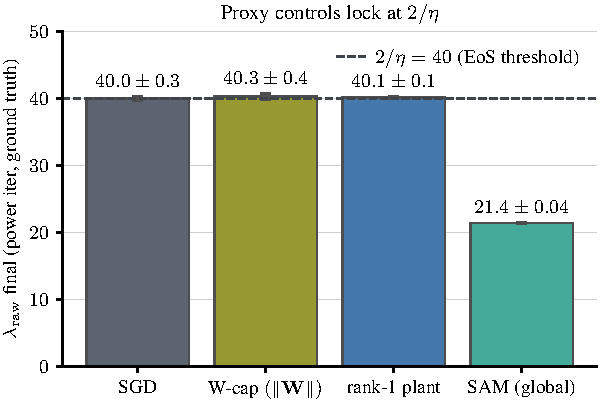
\includegraphics[width=0.62\linewidth]{26_multiseed_control_results.pdf}
\caption{多种子控制结果（论文图 26；误差棒为 $95\%$ CI，所有臂 $n{=}5$）：
W-帽（C1）与 free-lagged 秩-1 plant（体制 (i)）都锁在 $2/\eta$，只有全局
的 SAM 逃逸到下方。（精确 $\vtope$ 的秩-1 变体——体制 (ii)——反而上逃逸到
$2/\eta$ 之上，见图 \ref{fig:ch05-rankk}；$\gamma$-帽控制 C2 见正文。）}
\label{fig:ch05-control}
\end{figure}

\paragraph{体制 (ii)：accurate $\hat v$（精确估计）——精确抵消，帽被移除，上逃逸。}
把 $\hat v$ 换成热启动幂迭代的精确估计（即论文 rank-$k$ sweep（sweep，扫描）的 $k{=}1$
臂）：$\lmax^{\mathrm{final}}=261.8\pm5.4$。机制：抵消现在是精确的
（$\eta_{\mathrm{eff}}\lambda_{1}=2$；$\eta_{\mathrm{eff}}$ 为阻尼后
顶部方向的有效步长），周期-2 振荡被杀死，自稳定帽被移除
，渐进尖锐化无遮拦地把 $\lmax$ 推过 $2/\eta$——\textbf{上逃逸}，与控制
目标正好相反。

附带一个反直觉结果：上逃逸臂的 train loss 更低（$0.090$ vs $0.111$），
held-out 测试 MSE 也更低（$0.0932$ vs $0.1142$，$n{=}5$）——但最小值
\emph{更尖、不平坦}。锐度本身并没有换来泛化惩罚；论文讨论节的 Limitations
(vi) 对这一单任务反例做了 scope 限定。

\begin{figure}[!ht]
\centering
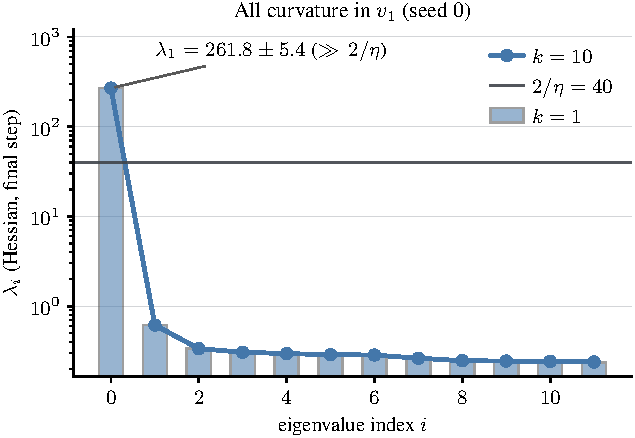
\includegraphics[width=0.62\linewidth]{27_rankk_sweep.pdf}
\caption{rank-$k$ sweep（sweep，扫描；论文图 27）：1-D sharp（一维
尖锐：谱里只有 $\lambda_1$ 一个尖方向）的 teacher--student 景观在
精确幂迭代 $\vtope$ 阻尼后的 top-12 海森谱（seed 0，$n{=}5$）。谱是
1-D sharp：$\lambda_{1}=261.8\pm5.4\gg2/\eta$ 而
$\lambda_{2}\approx0.6$——除 top 外无处可迁；$k{=}1,2,5,10$ 逐 bit 相同
，正是``帽移除''的预言（``迁移''则预言更多阻尼 $\Rightarrow$ 更低
$\lmax$，与观测相反）。}
\label{fig:ch05-rankk}
\end{figure}

图 \ref{fig:ch05-rankk} 同时为第 \ref{sec:ch07} 章埋下伏笔：迁移读法需要
第二个尖方向才有地方搬，而默认景观是 1-D sharp
（$\lambda_{1}=261.8\pm5.4\gg\lambda_{2}\approx0.6$）——所以论文干脆构造
一个两方向同钉 $2/\eta$ 的景观，在迁移唯一可能起作用的地方检验它。

\paragraph{``re-acquire $\vtope$''（重新获取/刷新特征向量）变体为何锁死在 $2/\eta$。}
该变体最终锁定 $40.019\pm0.002=2/\eta$，曾被读作``即使刷新特征向量也不逃
''的独立证据。真相是实现冗余：每步末刷新的 $\vtope$ 会在下一步被 free
$\Delta\theta$ 覆写（$\hat v\leftarrow\mathrm{unit}(\Delta\theta)$），于是
它除刷新后的单步外全程退化为 free-lagged 变体——体制 (i)，不是独立结局。
真正``每步精确 $\vtope$''的测试是带持久热启动的 rank-$k$ sweep（上一段）
，它落在体制 (ii)。研究日志（发现 23）把这次纠错列为必须主动承认的方法论
缺陷——论文以此为例展示了如何把一个看似支持自己的假证据识别并撤回。

\subsection{与教程的衔接：给自稳定振荡装上执行器的两种结局}
\label{sec:ch05-tutorial}

教程第 7 节展示了周期-2 振荡与自稳定化：$\lmax$ 爬到 $2/\eta$，Damian
三阶项把振荡振幅稳住，形成自稳定帽。本章做的事是\emph{用执行器干预它}，
并展示仅有的两种结局：阻尼不完美（体制 (i)）$\to$ 振荡留存 $\to$ 帽留存
$\to$ 钉在 $2/\eta$；阻尼精确（体制 (ii)）$\to$ 振荡被杀死 $\to$ 帽被移除
$\to$ 上逃逸过 $2/\eta$。唯独没有的结局是``压到 $2/\eta$ 以下''——单方向
阻尼做不到；只有 SAM 的全局扰动
（$\varepsilon=\rho\,\mathbf{g}/\|\mathbf{g}\|$，Foret 等 2021；SAM 的
两步算法与``全局''的数学含义见第~\ref{sec:ch01}~章的概念详解框）把均衡点
带到 $21.35\pm0.04<40$。为什么全局动作能而局部动作不能、这个排序如何扛过
四个压力测试，是第 \ref{sec:ch06}、\ref{sec:ch07} 章与解读第八章的主题。

\subsection*{本章要点}
\begin{itemize}
  \item \textbf{C1/C2：帽住 proxy 不动 $\lmax$。}权重范数帽频繁触发
        （$\sim750/3000$ 步）仍锁 $2/\eta$（$40.26\pm0.43$）；BN-$\gamma$
        帽不降反宽（$81.6\pm19.2$ vs $73.0\pm12.9$）且精度略差（$0.754$
        vs $0.768$）——相关性可作预测器、不可作执行器。
  \item \textbf{C3 体制 (i)：}free-lagged $\hat v$ 阻尼不完美，周期-2
        振荡与自稳定帽留存，$\lmax$ 钉在 $2/\eta$（$40.12\pm0.12$）；
        $\hat\lambda$ 塌缩到 $\sim10^{-4}$ 是 $\hat v$-跟踪失败，不是
        迁移签名。
  \item \textbf{C3 体制 (ii)：}精确 $\hat v$ 使
        $\eta_{\mathrm{eff}}\lambda_{1}=2$，振荡被杀死、帽被移除，上逃逸
        到 $261.8\pm5.4$——与控制目标相反；逃逸臂的 loss 与测试 MSE 反而
        更低（$0.090$/$0.0932$ vs $0.111$/$0.1142$），但最小值更尖。
  \item \textbf{``re-acquire'' 变体的 $40.019\pm0.002$}是覆写造成的退化
        （体制 (i)），不是独立证据——一个被主动撤回的假支持证据。
  \item \textbf{排序成立：}proxy 帽与单方向 plant 都不下逃逸，只有 SAM
        全局动作下行——该排序将经受四个压力测试
        （第 \ref{sec:ch07} 章与解读第八章）。
\end{itemize}
